\chapter{Grundlagen}
\label{cha:grundlagen}
In diesem Kapitel wird eine Übersicht über die verschiedenen Funktionsweisen gegeben. Darauf aufbauend wird dann herausgestellt, welche Art von Speicherung in diesem Projekt umgesetzt wird. Dabei wird auch auf die Unterschiedliche Auffassung des Begriffes \textit{Cache} eingegangen und die Unterschiede werden erläutert.

\section{Definition eines Caches}
\label{sec:cache-definition}
Ein \textit{Cache} wird im Allgemeinen als eine Speicherregion oder Puffer verstanden, die besonders schnell erreichbar sind. Darin werden oft verwendete Daten gespeichert, um höheren Speicherverbrauch gegen einen Performancegewinn zu tauschen.\\
\textit{Caches} werden in verschiedenen Umgebungen eingesetzt. Es wird zwischen \textit{Memory Cache}, \textit{Internet Browser Cache}, \textit{Disk Caching} und \textit{Server Caching} unterschieden.\\
Der \textit{Memory Cache} wird in Computern verwendet, um den sehr schnellen \ac{SRAM} des Rechners auszunutzen. Diese Art macht es sich zunutze, dass Programme immer dieselben Daten oder Befehle ausführen. Diese Ergebnisse werden dann vom Betriebssystem in diesem \textit{Cache} gespeichert, um zum Beispiel darauf aufbauend schnellere Berechnungen vollziehen zu können. Dieser Speicher wird dann dem dazu relativ langsamen \ac{DRAM} vorgezogen.\footcite[Vgl.][S.48f.]{Cache-GummerSommer}\\
Der \textit{Internet Browser Cache} wird ähnlich, aber in einem anderen Einsatz verwendet. Dieser speichert beliebte Seiten des Benutzers zwischen, um den Seitenaufruf zu beschleunigen. Dabei werden Dateien und \textit{Requests} zu der besuchten Seite gespeichert. Wenn man dann wieder zurück navigiert, kann der \textit{Browser} viele Dateien wiederverwenden und muss nicht mehr die gesamte Seite nachladen. Diese Variante wird auch \textit{Read Cache} genannt.\footcite{Cache-Techtarget}\\
\textit{Disk Caching} wird besonders beim Lesen von Festplatten verwendet. Dabei werden Daten im \textit{Memory Buffer}gespeichert. Dieser liegt heutzutage in einem gesonderten Bereich auf der Festplatte. Der Bereich kann sich jedoch auch im \ac{RAM} des Computer befinden.\footcite{Cache-Techtarget-DiskCache}\\
Beim \textit{Server Caching} geht es darum, den \textit{Traffic} in einem Netzwerk zu minimieren, indem die meistbesuchten Seiten auf einem \textit{Caching Server} gespeichert werden. Wenn ein Benutzer aus dem Netzwerk dann diese Seite aufruft, wird die Seite aus dem \textit{Cache} zurückgegeben und der \textit{Request} muss nicht wieder über das Internet geleitet werden, sondern wird direkt im internen Netzwerk beantwortet.\footcite{Cache-ProxyCache}\\

\subsection{Funktionsweisen von Caches}
\label{ssec:cache-funktionsweisen}
\textit{Caches} können in zwei unterschiedliche Funktionsweisen unterteilt werden, die im Folgenden genauer vorgestellt werden.

\subsubsection{Store Forward}
\label{sssec:cache-store-forward}
Das \textit{Store and Forward}-Prinzip ist eine spezielle Art des \textit{Cachings}, das Netze überbrücken soll, welche Verzögerungen tolerieren. Gegensätzlich dazu sind die Techniken \textit{Streaming} und Internettelefonie, die keine Verzögerungen tolerieren. Gleichzusetzen ist diese Technik mit der \ac{TCP}-Übertragung, die auch zwischengespeichert werden kann. Der Vorteil dieser Technik besteht darin, dass eine Zwischenstation die übertragenen Daten speichert, auf Integrität prüft und, wenn gewünscht, weiterleitet.\footcite{Cache-StoreForward}\\
Diese Technik kann auch in einem System untergebracht werden. So soll ein Datum auf der Festplatte gespeichert werden, wird dazu jedoch sicherheitshalber im Puffer zwischengespeichert. Direkt danach wird dieses Datum abgerufen, ist aber noch nicht auf die Festplatte geschrieben. Dann kann das Datum aus dem Puffer geladen werden und die geringe Geschwindigkeit der Festplatte wird dem Anwender nicht bewusst.\footcite{Cache-StoreForwardSOA}

\subsubsection{Function Cache}
\label{sssec:cache-function-cache}
Beim \textit{Function Cache} oder auch \textit{Memoization} handelt es sich um einen \textit{Cache}, der die Funktionsaufrufe eines Programmes samt Ergebnissen speichert. Diese werden dann in den meisten Fällen für darauf aufbauende Berechnungen oder Aktionen verwendet und sorgen somit für einen enormen Geschwindigkeitsanstieg.\footcite{Cache-Memoization}

%\subsection{Ersetzungsalgorithmen}
%\label{sssec:cache-ersetzungsalgorithmen}
%FIFO, LRU, LRU, Random

\subsection{Unsere Definition eines Caches}
\label{ssec:cache-unsere-definition}
Im Folgenden wird der Begriff des \textit{Caches} als eine abgewandelte Technik zur lokalen Zwischenspeicherung von Daten auf einem mobilen Gerät verstanden. Die allgemeine Definition geht bei einem \textit{Cache} von einer Perfomrancesteigerung aus (siehe Kapitel \ref{sec:cache-definition}), in diesem Projekt wird das Speichern von Daten jedoch dazu verwendet, um Daten auch offline zur Verfügung zu haben. Die bestehenden Eigenschaften zur Ersetzung von Daten und den verschiedenen Arten der Datenspeicherung werden beibehalten, jedoch im ersten Meilenstein nur rudimentär umgesetzt. Dabei wird eine Art \textit{Store and Forward} umgesetzt, jedoch wird bevorzugt auf den Server zugegriffen, da dieser als primärer Persistenzspeicher fungiert. Ein \textit{Function Cache} wird nicht umgesetzt, da dieser in diesem Anwendungsfall nicht optimal wäre. Es werden die Daten benötigt, die untereinander auch Beziehungen besitzen. Dabei reicht es nicht aus, die Funktionsaufrufe mit den entsprechenden Daten zu speichern, da man die gespeicherten Daten in einigen Fällen über mehrere Abfragen erhalten würde und diese dann mehrfach gespeichert werden würden. Dieses Problem würde dann die Effizienz des Zwischenspeicherns umgehen.

\section{Allgemeine Umsetzung des Caches}
\label{sec:cache-umsetzung}
Der \textit{Cache} wird in beiden Applikationen als eine lokale Datenbank umgesetzt und spiegelt die Datentypen des Servers in einem möglichst großen Umfang wider (siehe Kapitel \ref{sec:Datenbank-Entwurf} zum Aufbau der Server-Datenbank). Die genaue Umsetzung und Auswahl der Entitäten und Attribute muss entsprechend der Umsetzung und der technischen Möglichkeiten geschehen. Dabei wird jedoch weiterhin auf eine möglichst große Übereinstimmung zwischen den verschiedenen Applikationen geachtet. Somit sind die Entwicklungen besser zu vergleichen und bieten den Autoren damit ein besseres Maß zur Entscheidung, welche Applikation zu einem Messeprototypen weiterentwickelt wird.

\subsection{Aufbau des Caches}
\label{ssec:cache-aufbau}
Der \textit{Cache} als solches ist die Kombination aus der Logik, die in der Applikation zur Datenhaltung mit umgesetzt wird und einer lokalen Datenbank zur Speicherung der Daten. Die Schicht der \textit{Business}-Logik muss dabei Methoden zur Verfügung stellen, um die Daten lokal zu speichern und diese Daten dann auch wieder auslesen zu können.\\
Des Weiteren muss die Logik zur Synchronisierung von Daten zwischen der lokalen und der Server-Datenbank umgesetzt werden. Diese wird im Folgenden allgemein beschrieben.

\subsection{Funktionsweise des Caches}
\label{ssec:cache-unsere-funktionsweise}
Der \textit{Cache} muss die Daten auf demselben Stand halten, wie sie auf dem Server vorliegen. Deshalb bietet es sich an, Daten, die zum Server geschickt werden, auch lokal direkt zu speichern. Daten, die abgerufen werden, auch lokal zu speichern. Somit hat man keine unnötigen Abfragen zum Erhalt der Datenkonsistenz zwischen den beiden Ebenen. Diese Strategie hat somit einen positiven Einfluss auf die Performance der Applikationen und entlastet den Server von übermäßigen \textit{Requests}. In dem folgenden Sequenzdiagramm ist der Ablauf für die Logik des \textit{Caches} bei einem \textit{Get}-Aufruf an den Server zu sehen.

%CacheGet-Bild
\begin{figure}[h]
\centering
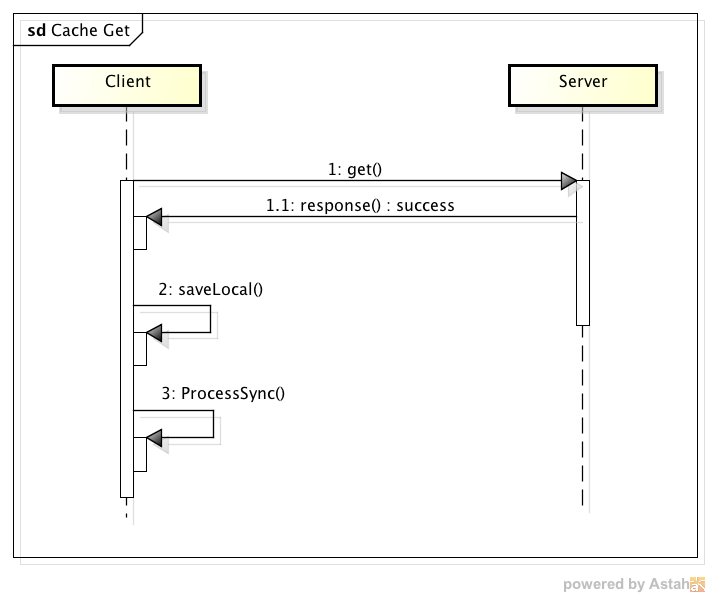
\includegraphics[width=0.8\linewidth]{content/images/Cache-Get}
\caption{Abrufen vom Server}
\label{pic:cacheGet}
\end{figure}

Die Synchronisation soll demnach im Anschluss einer Serververbindung geschehen, da man in diesem Fall sicher sein kann, dass eine Verbindung besteht, die dafür verwendet werden kann. Dementsprechend funktioniert auch der \textit{Post} oder das Hochladen von Daten (siehe Anhang \ref{sec:cachePost}).